\documentclass[12pt,letterpaper]{exam}
\usepackage[lmargin=1in,rmargin=1in,tmargin=1in,bmargin=1in]{geometry}
\usepackage{../style/exams}

% -------------------
% Course & Exam Information
% -------------------
\newcommand{\course}{MATH 141: Exam 3}
\newcommand{\term}{Fall --- 2024}
\newcommand{\examdate}{11/20/2024}
\newcommand{\timelimit}{75 Minutes}

\setbool{hideans}{false} % Student: True; Instructor: False

% Shaded Lines - Area Between Curves
\usepgfplotslibrary{fillbetween}
%\usetikzlibrary{patterns}

% -------------------
% Content
% -------------------
\begin{document}

\examtitle
\instructions{Write your name on the appropriate line on the exam cover sheet. This exam contains \numpages\ pages (including this cover page) and \numquestions\ questions. Check that you have every page of the exam. Answer the questions in the spaces provided on the question sheets. Be sure to answer every part of each question and show all your work. If you run out of room for an answer, continue on the back of the page --- being sure to indicate the problem number.} 
\scores
\bottomline
\newpage


% -------------------
% Questions
% -------------------
\begin{questions}

% Question 1
\newpage
\question[15] Consider the plot of a function $f(x)$ given below.
	\[
	\fbox{
	\begin{tikzpicture}[scale=1.2,every node/.style={scale=0.5}]
	\begin{axis}[
	grid=both,
	axis lines=middle,
	ticklabel style={fill=blue!5!white},
	xmin= -1.5, xmax=12.5,
	ymin= -5.5, ymax=8.5,
	xtick={-2,0,...,12},
	ytick={-6,-4,...,8},
	minor tick = {-10,-9,...,12},
	xlabel=\(x\),ylabel=\(y\),
	]
	\addplot[line width= 0.03cm,samples=5,domain= 0:2] ({x},{3*x});
	\addplot[line width= 0.03cm,samples=5,domain= 2:4] ({x},{12 - 3*x});
	\addplot[line width= 0.03cm,samples=5,domain= 4:8] ({x},{-3});
	\addplot[line width= 0.03cm,samples=70,domain= 8:12] ({x},{sqrt(4 - (x - 10)^2) + 4});
	
	\addplot[holdot] coordinates{(4,0)(8,-3)};
	\addplot[soldot] coordinates{(4,-3)(8,4)};
	
	\draw[draw=none,fill=red,opacity=0.2] (0,0) -- (4,0) -- (2,6) -- (0,0);
	\draw[draw=none,fill=blue,opacity=0.2] (4,0) -- (4,-3) -- (8,-3) -- (8,0) -- (4,0);
	\draw[draw=none,fill=green,opacity=0.2] (8,0) -- (12,0) -- (12,4) -- (8,4) -- (8,0);
	\draw[draw=none,fill=yellow,opacity=0.4] (12,4) arc (0:180:2);
	
	\node at (2,2) {\Large$A_1= 12$};
	\node at (6,-1.6) {\Large$A_2= 12$};
	\node at (10,2) {\Large$A_3= 8$};
	\node at (10,4.8) {\Large$A_4= 2\pi$};
	\end{axis}
	\end{tikzpicture}
	}
	\]
Using the above plot, compute the following: \par\vspace{0.3cm}
	\begin{enumerate}[(a)]
	\item $\displaystyle\int_0^8 f(x) \;dx= A_1 + (-A_2)= \dfrac{1}{2}\,4(6) - 4(3)= 12 - 12= 0$ \pspace\pspace\vfill
	
	\item $\displaystyle\int_8^{12} f(x) \;dx= A_3 + A_4= 4(4) + \frac{1}{2} \pi (2^2)= 16 + 2\pi \approx 22.2832$ \pspace\pspace\vfill
	
	\item $\displaystyle\int_0^{12} f(x) \;dx= \int_0^8 f(x) \;dx + \int_8^{12} f(x) \;dx= 0 + (16 + 2\pi)= 16 + 2\pi \approx 22.2832$ \pspace\pspace\vfill
	
	\item $\displaystyle\int_6^6 f(x) \;dx= 0$ \pspace\pspace\vfill
	
	\item The area between $f(x)$ and the $x$-axis. \pspace
		\[
		A_1 + A_2 + (A_3 + A_4)= 12 + 12 + (16 + 2\pi)= 40 + 2\pi \approx 46.2832
		\] \vfill
	\end{enumerate}



% Question 2
\newpage
\question[10] Showing all your work, compute the following: \par\vspace{0.3cm}
	\begin{enumerate}[(a)]
	\item $\ds\int \left(\sin x - 5^x + 3 \tan x \right) \;dx$ \par\vspace{0.2cm}\vfill
		
		\[
		\int \left(\sin x - 5^x + 3 \tan x \right) \;dx= -\cos x - \dfrac{5^x}{\ln 5} + 3 \ln|\sec x| + C
		\] \pspace
		
		\begin{center} OR \end{center}
		
		\[
		\int \left(\sin x - 5^x + 3 \tan x \right) \;dx= -\cos x - \dfrac{5^x}{\ln 5} - 3 \ln|\cos x| + C
		\] \vfill
	
	\item $\ds\int_0^1 \left( \dfrac{1}{\sqrt{x}} - e^x \right) \;dx$ \vfill
		
		\[
		\begin{aligned}
		\int_0^1 \left( \dfrac{1}{\sqrt{x}} - e^x \right) \;dx&= \int_0^1 \left( x^{-1/2} - e^x \right) \;dx \\[0.2cm]
		&= 2x^{1/2} - e^x \bigg|_0^1 \\[0.2cm]
		&= \big( 2(1) - e^1 \big) - \big( 2(0) - e^0 \big) \\[0.2cm]
		&= (2 - e) - (-1) \\[0.2cm]
		&= 3 - e
		\end{aligned}
		\] \vfill
	\end{enumerate}



% Question 3
\newpage
\question[10] Showing all your work, compute the following: \par\vspace{0.3cm}
	\begin{enumerate}[(a)]
	\item $\ds \dfrac{d}{dx} \int_{e^x}^\pi \dfrac{\arcsin(t)}{1 + t^2} \;dt$ \par\vspace{1cm} \vfill
	
		\[
		\dfrac{d}{dx} \int_{e^x}^\pi \dfrac{\arcsin(t)}{1 + t^2} \;dt= \dfrac{d}{dx} \left( -\int_\pi^{e^x} \dfrac{\arcsin(t)}{1 + t^2} \;dt \right)= -\dfrac{\arcsin(e^x)}{1 + (e^x)^2} \cdot e^x= \dfrac{-e^x \arcsin(e^x)}{1 + e^{2x}}
		\] \par\vspace{1cm} \vfill
	\item $\ds \dfrac{d}{dx} \int_{-2}^{\sec(5x)} \ln \left( \dfrac{1 - t}{1 + t} \right) \;dt$ \vfill
	
		\[
		\hspace{-2.5cm} \dfrac{d}{dx} \int_{-2}^{\sec(5x)} \ln \left( \dfrac{1 - t}{1 + t} \right) \;dt= \ln \left( \dfrac{1 - \sec(5x)}{1 + \sec(5x)} \right) \cdot \sec(5x) \tan(5x) \cdot 5= 5 \sec(5x) \tan(5x) \ln \left( \dfrac{1 - \sec(5x)}{1 + \sec(5x)} \right)
		\] \vfill
	
	{\itshape\tiny Note. Using the half-angle identity $\tan \left( \frac{\theta}{2} \right)= \frac{1 - \cos \theta}{\sin \theta}$, we have $\frac{1 - \sec 5x}{1 + \sec 5x} \cdot \frac{\cos 5x}{\cos 5x}= \frac{\cos 5x - 1}{\cos 5x + 1} \cdot \frac{1 - \cos 5x}{1 + \cos 5x}= \frac{-(1 - \cos 5x)^2}{1 - \cos^2 5x}= - \frac{(1 - \cos 5x)^2}{\sin^2 5x}= -\left( \frac{1 - \cos 5x}{\sin 5x} \right)^2= -\tan^2 \left( \frac{5x}{2} \right)$. Therefore, the answer above can be expressed as $5 \sec(5x) \tan(5x) \ln \left( -\tan^2 \left(\frac{5x}{2} \right) \right)$.}
	\end{enumerate}



% Question 4
\newpage
\question[10] Showing all your work, compute the following:
	\[
	\int \dfrac{dx}{5x^2 + 16}
	\] \pspace

{\itshape \tsol We have\dots 
	\[
	\begin{aligned}
	\int \dfrac{dx}{5x^2 + 16}&= \int \dfrac{dx}{5x^2 + 16} \cdot \dfrac{1/16}{1/16} \\[0.3cm]
	&= \dfrac{1}{16} \int \dfrac{dx}{ \frac{5}{16}\,x^2 + 1} \\[0.3cm]
	&= \dfrac{1}{16} \int \dfrac{dx}{ \left( \frac{\sqrt{5}}{4} \,x \right)^2 + 1} 
	\end{aligned}
	\]
Now we make a substitution: 
	\[
	\begin{aligned}
	u= \frac{\sqrt{5}}{4}\,x \\[0.5cm]
	du= \dfrac{\sqrt{5}}{4}\;dx \\[0.1cm]
	dx= \dfrac{4}{\sqrt{5}}\;du
	\end{aligned}
	\]
But then, we have\dots
	\[
	\begin{aligned}
	\int \dfrac{dx}{5x^2 + 16}&= \dfrac{1}{16} \int \dfrac{dx}{ \left( \frac{\sqrt{5}}{4} \,x \right)^2 + 1} \\[0.3cm]
	&= \dfrac{1}{16} \int \dfrac{4/\sqrt{5}}{u^2 + 1} \;du \\[0.3cm]
	&= \dfrac{4}{16 \sqrt{5}} \int \dfrac{du}{u^2 + 1} \\[0.3cm]
	&= \dfrac{1}{4\sqrt{5}}\, \arctan u + C \\[0.3cm]
	&= \dfrac{1}{4\sqrt{5}}\, \arctan \left( \dfrac{\sqrt{5}}{4}\,x \right) + C
	\end{aligned}
	\]
}



% Question 5
\newpage
\question[10] Consider the region, $\mathcal{R}$, shown below.
	\[
	\fbox{
	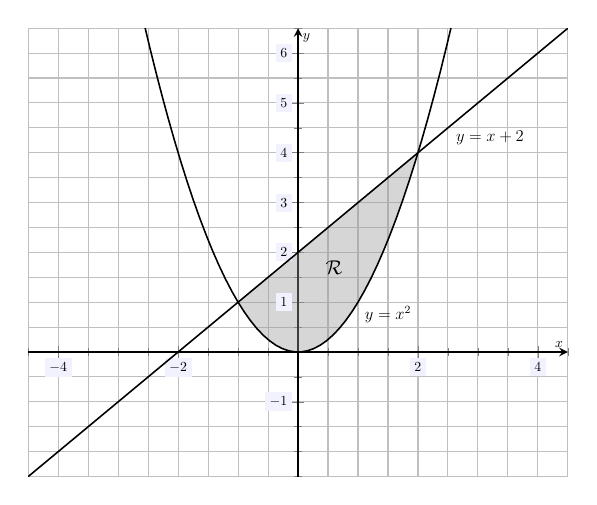
\begin{tikzpicture}[scale=1,every node/.style={scale=0.5}]
	\begin{axis}[
	grid=both,
	axis lines=middle,
	ticklabel style={fill=blue!5!white},
	xmin= -4.5, xmax=4.5,
	ymin= -2.5, ymax=6.5,
	xtick={-8,-6,...,8},
	ytick={-1,0,...,8},
	minor tick = {-8,-7.5,...,8},
	xlabel=\(x\),ylabel=\(y\),
	]
	\node at (1.5,0.75) {\large$y= x^2$};
	\addplot[name path=F,line width= 0.02cm,samples=5,domain= -10.5:10.5] ({x},{x + 2});
	\node at (3.2,4.3) {\large$y= x + 2$};
	\addplot[name path=G,line width= 0.02cm,samples=200,domain= -10.5:10.5] ({x},{x^2});
	\addplot[color=gray!80,opacity=0.4] fill between[of= F and G, soft clip={domain= -1:2}];
	\node at (0.6,1.7) {\Large$\mathcal{R}$};
	\end{axis}
	\end{tikzpicture}
	}
	\] 

\begin{enumerate}[(a)]
\item \scalebox{1}{Set-up \textit{but do not evaluate} an integral with respect to $x$ that computes the area of $\mathcal{R}$.} \par\vspace{1.1cm}\vfill

	\[
	\int_{-1}^2 \big( (x + 2) - x^2 \big) \;dx
	\] \par\vspace{1.1cm}\vfill
	
\item \scalebox{1}{Set-up \textit{but do not evaluate} an integral with respect to $y$ that computes the area of $\mathcal{R}$.} \vfill

{\itshape Observe that if $y= x^2$, then $x= \pm \sqrt{y}$, where $x= -\sqrt{y}$ if $x < 0$ and $x= \sqrt{y}$ if $x \geq 0$. Finally, observe that if $y= x + 2$, then $x= y - 2$. Therefore, we have\dots} \par\vspace{0.75cm}

	\[
	\int_0^1 \big( \sqrt{y} - (-\sqrt{y}) \big) \;dy + \int_1^4 \big( \sqrt{y} - (y - 2) \big) \;dy
	\] \vfill

{\itshape \scriptsize Note. The area of the region, hence the final value of both parts above, is $\frac{9}{2}$.}
\end{enumerate}



% Question 6
\newpage
\question[10] Showing all your work, compute the following:
	\[
	\int_0^2 \dfrac{3x}{x^2 + 1} \;dx
	\] \pspace

{\itshape \tsol We have\dots
	\[
	\begin{aligned}
	u&= x^2 + 1 \\[0.4cm]
	du&= 2x \;dx \\
	dx&= \dfrac{1}{2x} \;du
	\end{aligned}
	\qquad\qquad
	\begin{aligned}
	x=2 \colon u= 2^2 + 1= 5 \\
	x=0 \colon u= 0^2 + 1= 1
	\end{aligned}
	\]
But then, we have\dots
	\[
	\begin{aligned}
	\int_0^2 \dfrac{3x}{x^2 + 1} \;dx&= 3 \int_0^2 \dfrac{1}{x^2 + 1} \cdot x\; dx \\[0.3cm]
	&= \dfrac{3}{2} \int_0^2 \dfrac{1}{x^2 + 1} \cdot 2x\; dx \\[0.3cm] 
	&= \dfrac{3}{2} \int_1^5 \dfrac{1}{u} \;du \\[0.3cm]
	&= \dfrac{3}{2} \ln|u| \;\bigg|_1^5 \\[0.3cm]
	&= \dfrac{3}{2} \cdot \left( \ln(5) - \ln(1) \right) \\[0.3cm]
	&= \dfrac{3}{2} \, \ln(5) 
	\end{aligned}
	\] \vfill

Note. One could also express the answer as $\frac{3}{2} \, \ln(5)= \ln(5^{3/2})= \ln(\sqrt{125})$.
}



% Question 7
\newpage
\question[15] Showing all your work, approximate the integral below using a left-hand sum with three evenly spaced rectangles \textit{but do not evaluate or simplify this sum}.
	\[
	\int_1^{13} \left( x \ln x - 1 \right) \;dx
	\] \pspace

{\itshape \tsol We can create a plot of this approximation---the plot need not be accurate, merely `useful.' Because these rectangles are equally spaced, we know they each have width\dots
	\[
	\Delta x= \dfrac{b - a}{n}= \dfrac{13 - 1}{3}= \dfrac{12}{3}= 4
	\]
But then, we know that\dots
	\[
	\int_1^{13} \left( x \ln x - 1 \right) \;dx \approx 4 f(1) + 4f(5) + 4f(9)= 4 (\ln 1 - 1) + 4 (5 \ln 5 - 1) + 4 (9 \ln 9 - 1)
	\] \vfill

{\scriptsize Note. If one were to simplify the expression, one would have $4(9 \ln 9 + 5 \ln 5 - 3) \approx 99.2888$. The exact value of the integral is $\frac{169 \ln(169)}{4} - 54 \approx 162.738$. Therefore, this estimate has only a 39.99\% error using only three rectangles. Using ten, equally spaced left-hand rectangles would result in an estimate of 143.037---a 12.11\% error---and using one-hundred such rectangles would result in an estimate of 160.741---a 1.23\% error.}
}



% Question 8
\newpage
\question[10] Set-up \textit{but do not evaluate} an integral which computes the area between $f(x)= 3x + 4$ and $g(x)= 8 - x^2$. \pspace

{\itshape \tsol First, we create a rough sketch of the region. 
	\[
	\fbox{
	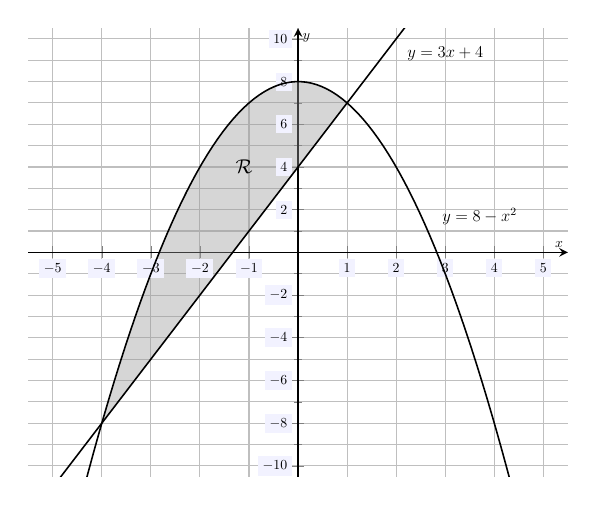
\begin{tikzpicture}[scale=1,every node/.style={scale=0.5}]
	\begin{axis}[
	grid=both,
	axis lines=middle,
	ticklabel style={fill=blue!5!white},
	xmin= -5.5, xmax=5.5,
	ymin= -10.5, ymax=10.5,
	xtick={-5,-4,...,5},
	ytick={-10,-8,...,10},
	minor tick = {-10,-9,...,10},
	xlabel=\(x\),ylabel=\(y\),
	]
	\node at (3.7,1.7) {\large$y= 8 - x^2$};
	\addplot[name path=F,line width= 0.02cm,samples=5,domain= -10.5:10.5] ({x},{3*x + 4});
	\node at (3,9.3) {\large$y= 3x + 4$};
	\addplot[name path=G,line width= 0.02cm,samples=200,domain= -10.5:10.5] ({x},{8 - x^2});
	\addplot[color=gray!80,opacity=0.4] fill between[of= F and G, soft clip={domain= -4:1}];
	\node at (-1.1,4) {\Large$\mathcal{R}$};
	\end{axis}
	\end{tikzpicture}
	}
	\] 
We need to find the intersection of the curves. We have\dots
	\[
	\begin{gathered}
	3x + 4= 8 - x^2 \\
	x^2 + 3x - 4= 0 \\
	(x + 4)(x - 1)= 0 
	\end{gathered}
	\]
This implies that either $x + 4= 0$, which implies $x= -4$, or $x - 1= 0$, which implies that $x= 1$. Using $x= 0$, observe that either $y= 8 - 0^2= 8$ or $y= 3(0) + 4= 4$. Therefore, the curve $y= 8 - x^2$ is `on top' on the interval $[-4, 1]$. Setting up the integral with respect to $x$, we have\dots
	\[
	\int_{-4}^1 \big( (8 - x^2) - (3x + 4) \big) \;dx
	\] \pspace
Alternatively, if $y= 3x + 4$, then $x= \frac{y - 4}{3}$, and if $y= 8 - x^2$, then $x= \pm \sqrt{8 - y}$, where $x= \sqrt{8 - y}$ if $x \geq 0$ and $x= -\sqrt{8 - y}$ if $x < 0$. Now if $x= -4$, we know that $y= 3(-4) + 4= -8$. If $x= 1$, we know that $y= 3(1) + 4= 7$. Using $y= 0$, we know that $x= \frac{0 - 4}{3}= -\frac{4}{3}$ and $x= \sqrt{8 - 0}= \sqrt{8}$. Therefore, $x= \sqrt{8 - y}$ is the curve `on the right' on the interval $[-8, 7]$. Setting up the integral with respect to $y$, we have\dots
	\[
	\int_{-8}^7 \left( \dfrac{y - 4}{3} - (-\sqrt{8 - y}) \right) \;dy + \int_7^8 \big( \sqrt{8 - y} - (-\sqrt{8 - y}) \big) \;dy
	\] \vfill

{\scriptsize Note. If one computes either of the integral expression above to compute the area of the region, one finds an area of $\frac{125}{6}$.}
}



% Question 9
\newpage
\question[10] Showing all your work, compute the following: \par\vspace{0.3cm}
	\begin{enumerate}[(a)]
	\item $\ds\int_{\pi/4}^{\pi/2} \cot x \csc x \;dx$ \vfill
		
		\[
		\int_{\pi/4}^{\pi/2} \cot x \csc x \;dx= -\csc x \bigg|_{\pi/4}^{\pi/2}= -\csc\left( \frac{\pi}{2} \right) - \left(- \csc \left( \dfrac{\pi}{4} \right) \right)= -1 - (-\sqrt{2})= \sqrt{2} - 1
		\] \vfill
	
	\item $\ds\int \left( 3 \cos x - \dfrac{x^3 + 6\sqrt{x}}{\sqrt{x}} \right) \;dx$ \vfill
	
		\[
		\int \left( 3 \cos x - \dfrac{x^3 + 6\sqrt{x}}{\sqrt{x}} \right) \;dx= \int \left( 3 \cos x -  x^{5/2} - 6 \right) \;dx= 3 \sin x - \dfrac{2}{7}\, x^{7/2} - 6x + C
		\] \vfill
	
	{\itshape\tiny Note. For (a), one can also use $u$-substitution with $u= \csc x$, so that $du= -\csc x \cot x \;dx$. If $x= \frac{\pi}{2}$, then $u= 1$, and if $x= \frac{\pi}{4}$, then $u= \sqrt{2}$. This results in the integral $\ds\int_{\sqrt{2}}^1 -1 \;du= -u \big|_{\sqrt{2}}^1= -1 - (-\sqrt{2})= \sqrt{2} - 1$. Alternatively, one can write the integrand as $\cot x \csc x= \frac{\cos x}{\sin x} \cdot \frac{1}{\sin x}= \frac{\cos x}{\sin^2 x}$. One can then choose $u= \sin x$, so that $du= \cos x \;dx$. If $x= \frac{\pi}{2}$, $u= 1$, and if $x= \frac{\pi}{4}$, then $u= \frac{1}{\sqrt{2}}$. This results in the integral $\int_{1/\sqrt{2}}^1 \frac{du}{u^2}= -\frac{1}{u} \big|_{1/\sqrt{2}}^1= -1 - \frac{-1}{1/\sqrt{2}}= \sqrt{2} - 1$.}
	\end{enumerate}


\end{questions}
\end{document}